\lstdefinelanguage{plaintext}{
  sensitive=false,
  comment=[l]{//},
  morecomment=[s]{/*}{*/},
  identifierstyle=\color{black},
  morestring=[b]',
  morestring=[b]"
}

\lstset
{ 
    language=plaintext,
    basicstyle=\footnotesize,
    numbers=left,
    stepnumber=1,
    showstringspaces=false,
    tabsize=1,
    breaklines=true,
    breakatwhitespace=false,
    frame=leftline
}

\chapter{Implementasi dan Pengujian}
\label{chap:implementasiDanPengujian}

Pada bab ini dibahas mengenai implementasi perangkat lunak dan pengujian yang dilakukan terhadap perangkat lunak tersebut. Lingkungan implementasi, yang meliputi perangkat keras dan perangkat lunak, serta hasil implementasi akan dijelaskan pada bab ini. Selain Pengujian yang dilakukan pada skripsi ini, yang meliputi pengujian fungsional dan eksperimental akan dijelaskan pada bab ini.

\section{Implementasi}
Pada bagian ini akan dijelaskan mengenai lingkungan yang digunakan untuk membangun perangkat lunak beserta hasil implementasinya.

\subsection{Lingkungan Implementasi}
Berikut spesifikasi perangkat keras dan perangkat lunak yang digunakan dalam pembangunan pada skripsi ini:

\begin{enumerate}
	\item Spesifikasi Perangkat Keras
	
		\begin{itemize}
			\item Perangkat: Laptop
			\item Processor: AMD Bristol Ridge Quad Core FX-9830P 3GHz
			\item RAM: 8GB
			\item GPU: Radeon RX 460
			\item Storage: Harddisk 1TB
		\end{itemize}		

	\item Spesifikasi Perangkat Lunak

		\begin{itemize}
			\item Sistem Operasi Windows 10 64-bit
			\item PHP 7.3.5 (cli)
			\item Composer versi 1.8.5
			\item Sublime Text versi 3.2.1
		\end{itemize}	
	
\end{enumerate}

\subsection{Hasil Implementasi}
Perangkat lunak dibangun menggunakan bahasa pemrograman \textit{PHP} dan \textit{library PdfParser}. Perangkat lunak tidak memiliki \textit{Graphical User Interface}, sehingga seluruh kegiatan dilakukan melalui terminal. Perangkat lunak akan menerima input berupa file PDF skripsi yang disimpan pada folder yang telah disediakan, dan mengeluarkan laporan kesalahan pada terminal.

\begin{lstlisting}[caption={Perintah yang digunakan untuk menjalankan perangkat lunak}	\label{lst:command},language=php,xleftmargin=.3\textwidth] 
php main.php ../res/nama_file.pdf
\end{lstlisting}
\medskip

Listing \ref{lst:command} merupakan perintah yang perlu dituliskan pada terminal, untuk menjalankan perangkat lunak. Kelas Main menjadi kelas yang digunakan untuk menjalankan seluruh proses yang berjalan dalam perangkat lunak. File PDF skripsi yang akan diperiksa harus berada di folder yang telah disediakan, yaitu pada folder Skripsi$\backslash$src$\backslash$res. Nama file yang digunakan pada umumnya sesuai dengan \textit{template} skripsi yang diberikan, yaitu ''skripsi.pdf''. Namun pengguna juga dapat menggunakan nama yang berbeda, yang paling utama file tersebut memiliki ekstensi PDF.

\begin{figure}[H]
	\centering	
	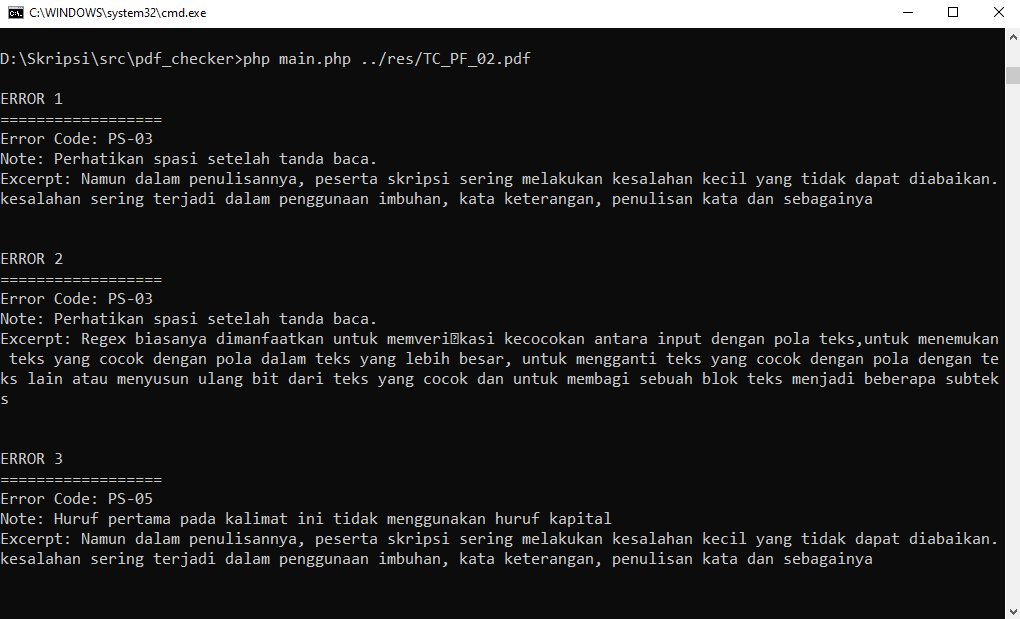
\includegraphics[scale=0.6]{hasil-implementasi.png}
	\caption{Laporan Kesalahan}	
	\label{fig:error_report} 
\end{figure}
\medskip

Gambar \ref{fig:error_report} merupakan hasil laporan yang dikeluarkan oleh perangkat lunak melalui \textit{terminal windows}. Informasi yang diberikan oleh laporan tersebut yaitu, kode kesalahan, jenis kesalahan yang ditemukan dan kesalahan yang ditemukan. Laporan kesalahan yang dikeluarkan sudah diurutkan dari fitur pertama hingga terakhir, yaitu dari fitur PS-01 hingga NAT-03.

\section{Pengujian Fungsional}
Pengujian fungsional bertujuan untuk menguji fungsionalitas perangkat lunak. Perangkat lunak memiliki 8 fitur yang telah diimplementasikan. Fitur-fitur tersebut akan diuji untuk melihat kebenaran dan kesesuaian fitur tersebut dengan yang diharapkan. Untuk melakukan pengujian ini, perangkat lunak akan dijalankan sebanyak jumlah fitur yang ada. Setiap pengujian yang dilakukan, fitur yang diaktifkan hanya 1 saja secara bergantian. Hal ini dilakukan hingga seluruh fitur telah diuji.

Pada pengujian ini, perangkat lunak akan diuji dengan 2 buah \textit{test case} dokumen skripsi Informatika Unpar dengan mode sidang akhir. Kedua \textit{test case} yang digunakan yaitu, ''TC\_PF\_01.pdf'' dan ''TC\_PF\_02.pdf''. Isi dari ke-2 file tersebut sama, namun pada file ''TC\_PF\_02.pdf'' sudah disisipkan kesalahan-kesalahan yang dapat dideteksi oleh setiap fitur yang ada. Berikut ini adalah rincian dari kesalahan-kesalahan yang dimasukan ke dalam \textit{test case} tersebut.

\begin{enumerate}
	\item Pada halaman cover bahasa Indonesia dan bahasa Inggris, data yang meliputi judul, nama mahasiswa, npm mahasiswa, dan yang lainnya tidak diisi. Hal ini dilakukan untuk menguji fitur pemeriksa kelengkapan data skripsi (KAL-03).
	
	\item Pada bab 1, hampir seluruh karakter pertama dalam kalimat menggunakan huruf kecil. Hal ini dilakukan untuk menguji fitur pemeriksa huruf kapital (PS-05).
	
	\item Pada bab 2, terdapat 2 buah teori yang referensinya tidak dirujuk dengan baik. Hal ini dilakukan untuk menguji fitur pemeriksa referensi (NAT-01).
	
	\item Pada bab 3, terdapat beberapa kata yang diketik tidak sesuai dengan kamus. Hal ini dilakukan untuk menguji fitur pemeriksa kata (PS-01). Selain itu pada bab ini tidak diberikan kata pengantar sebelum memulai subbab, untuk menguji fitur pemeriksa kata pengantar pada bab (KAL-02).
	
	\item Pada bab 4, terdapat beberapa kata yang tidak diberikan karakter spasi sebelum ataupun setelah tanda baca. Hal ini dilakukan untuk menguji fitur pemeriksa karakter spasi sebelumm atau setelah tanda baca (PS-03).	

	\item Untuk menguji fitur pemeriksa jumlah sub bab atau sub sub bab (PS-09), pada beberapa bab hanya memiliki sebuah sub bab atau sebuah sub sub bab.
		
	\item Pada bab 6, terdapat kalimat yang disisipkan kata ganti orang , untuk menguji fitur pemeriksa kata ganti orang (VAN-03).
\end{enumerate}

\subsection{Menguji fitur PS-01}
Hasil yang diharapkan dari pengujian fitur ini adalah perangkat lunak dapat menemukan kata-kata yang tidak terdapat pada kamus bahasa Indonesia \textit{LibreOffice}. Laporan kesalahan yang ditemukan pada \textit{test case} ''TC\_PF\_02.pdf'' dapat dilihat pada gambar \ref{fig:ujips01}.

\begin{figure}[H]
	\centering	
	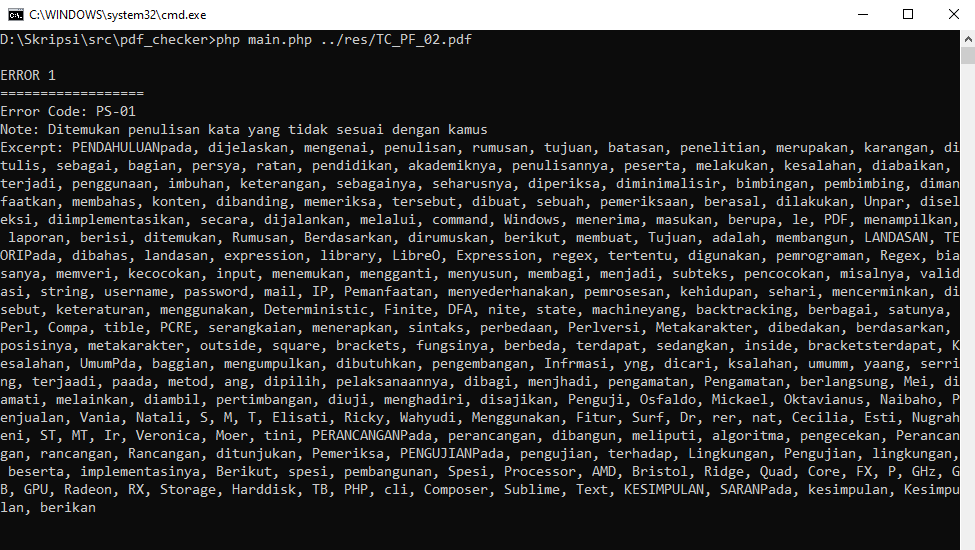
\includegraphics[scale=0.63]{uji_ps01.png}
	\caption{Laporan kesalahan fitur PS-01}	
	\label{fig:ujips01} 
\end{figure}

Laporan yang ditunjukan pada gambar \ref{fig:ujips01} sudah sesuai dengan yang diharapkan. Fitur ini melakukan pengecekan pada setiap kata yang ada pada dokumen. Namun fitur ini belum dapat membedakan kata yang termasuk nama orang, nama tempat, nama barang, kata yang berimbuhan dan kata yang menggunakan bahasa asing.

\subsection{Menguji fitur PS-03}
Hasil yang diharapkan dari pengujian fitur ini adalah perangkat lunak dapat menemukan kata-kata yang tidak diberi spasi setelah tanda baca. Laporan kesalahan yang ditemukan pada \textit{test case} ''TC\_PF\_02.pdf'' dapat dilihat pada gambar \ref{fig:ujips03}.

\begin{figure}[H]
	\centering	
	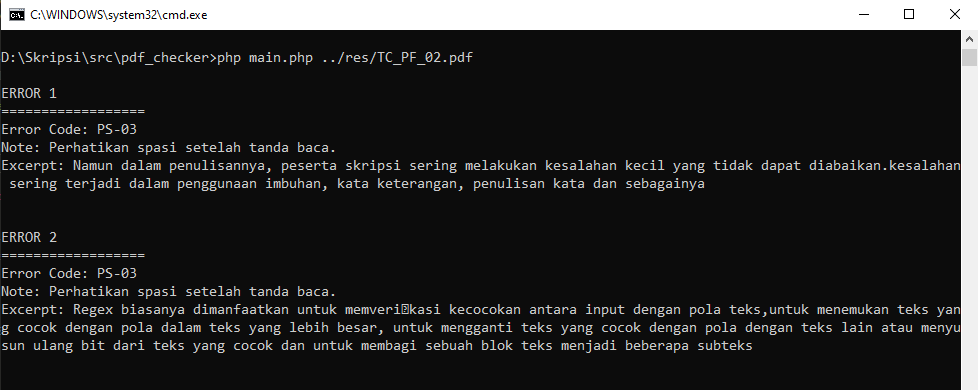
\includegraphics[scale=0.63]{uji_ps03.png}
	\caption{Laporan kesalahan fitur PS-03}	
	\label{fig:ujips03} 
\end{figure}

Laporan yang ditunjukan pada gambar \ref{fig:ujips03} sudah sesuai dengan yang diharapkan. Fitur ini masih belum bisa membedakan penggunaan tanda titik pada gelar pendidikan, perangkat lunak mendeteksi hal tersebut menjadi sebuah kesalahan dalam fitur ini.

\subsection{Menguji fitur PS-05}
Hasil yang diharapkan dari pengujian fitur ini adalah perangkat lunak dapat menemukan karakter pertama yang tidak menggunakan huruf kapital pada sebuah kalimat. Laporan kesalahan yang ditemukan pada \textit{test case} ''TC\_PF\_02.pdf'' dapat dilihat pada gambar \ref{fig:ujips05}.

\begin{figure}[H]
	\centering	
	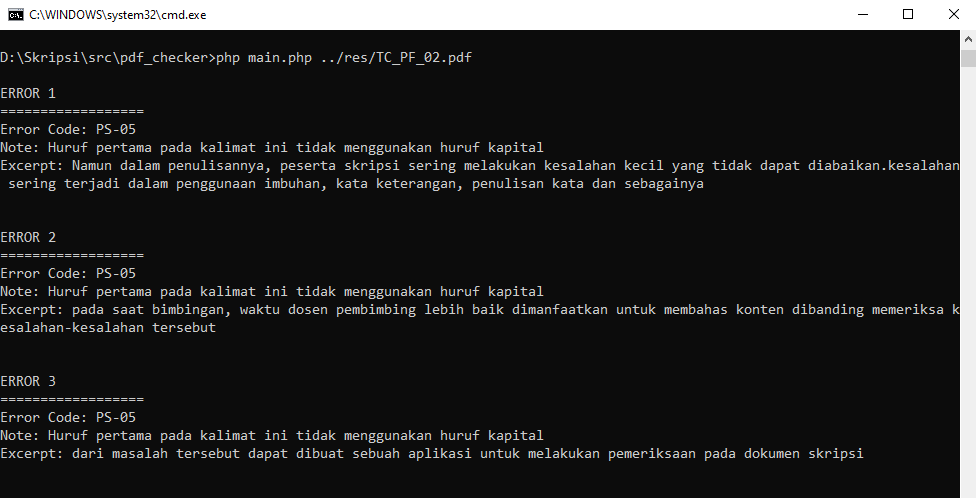
\includegraphics[scale=0.63]{uji_ps05.png}
	\caption{Laporan kesalahan fitur PS-05}	
	\label{fig:ujips05} 
\end{figure}

Laporan yang ditunjukan pada gambar \ref{fig:ujips05} sudah sesuai dengan yang diharapkan.

\subsection{Menguji fitur PS-09}
Hasil yang diharapkan dari pengujian fitur ini adalah perangkat lunak dapat menemukan bab atau sub bab yang hanya memiliki satu sub bab atau sub sub bab. Laporan kesalahan yang ditemukan pada \textit{test case} ''TC\_PF\_02.pdf'' dapat dilihat pada gambar \ref{fig:ujips09}.

\begin{figure}[H]
	\centering	
	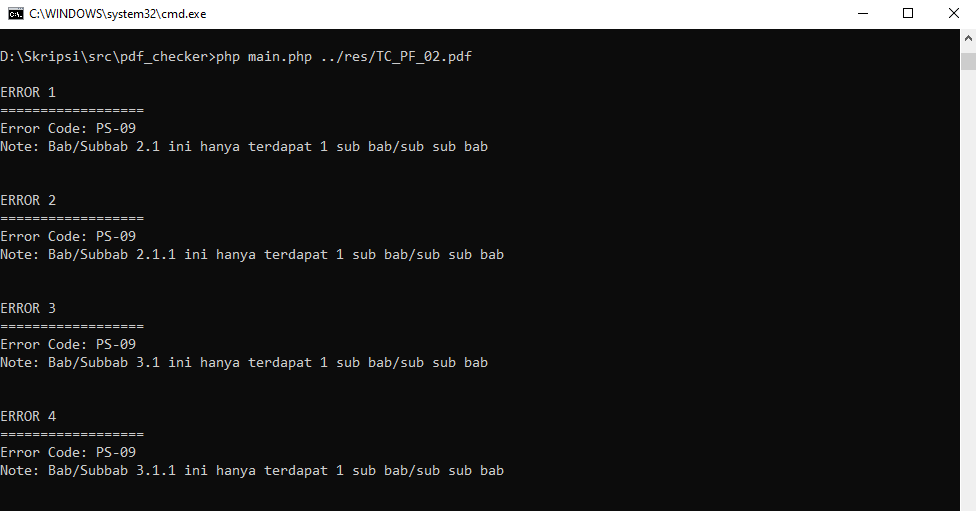
\includegraphics[scale=0.63]{uji_ps09.png}
	\caption{Laporan kesalahan fitur PS-09}	
	\label{fig:ujips09} 
\end{figure}

Laporan yang ditunjukan pada gambar \ref{fig:ujips09} sudah sesuai dengan yang diharapkan.

\subsection{Menguji fitur KAL-02}
Hasil yang diharapkan dari pengujian fitur ini adalah perangkat lunak dapat menemukan bab yang tidak diberikan kata pengantar. Laporan kesalahan yang ditemukan pada \textit{test case} ''TC\_PF\_02.pdf'' dapat dilihat pada gambar \ref{fig:ujikal02}.

\begin{figure}[H]
	\centering	
	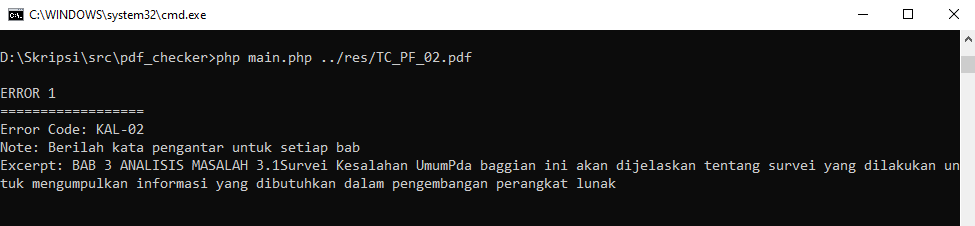
\includegraphics[scale=0.63]{uji_kal02.png}
	\caption{Laporan kesalahan fitur KAL-02}	
	\label{fig:ujikal02} 
\end{figure}

Laporan yang ditunjukan pada gambar \ref{fig:ujikal02} sudah sesuai dengan yang diharapkan.

\subsection{Menguji fitur KAL-03}
Hasil yang diharapkan dari pengujian fitur ini adalah perangkat lunak dapat menemukan data skripsi yang belum diisi. Laporan kesalahan yang ditemukan pada \textit{test case} ''TC\_PF\_02.pdf'' dapat dilihat pada gambar \ref{fig:ujikal03}.

\begin{figure}[H]
	\centering	
	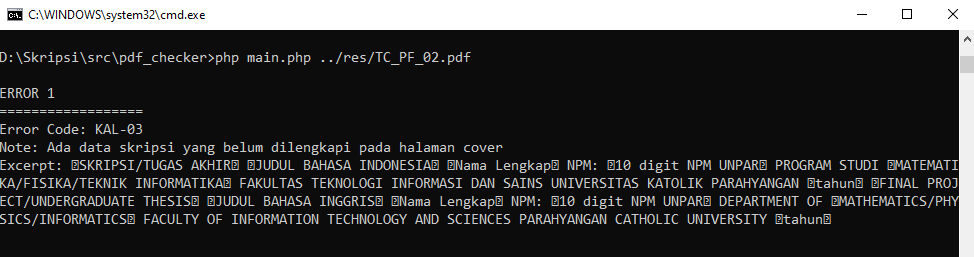
\includegraphics[scale=0.63]{uji_kal03.png}
	\caption{Laporan kesalahan fitur KAL-03}	
	\label{fig:ujikal03} 
\end{figure}

Laporan yang ditunjukan pada gambar \ref{fig:ujikal03} sudah sesuai dengan yang diharapkan.

\subsection{Menguji fitur NAT-01}
Hasil yang diharapkan dari pengujian fitur ini adalah perangkat lunak dapat menemukan referensi yang tidak dirujuk dengan baik. Laporan kesalahan yang ditemukan pada \textit{test case} ''TC\_PF\_02.pdf'' dapat dilihat pada gambar \ref{fig:ujinat01}.

\begin{figure}[H]
	\centering	
	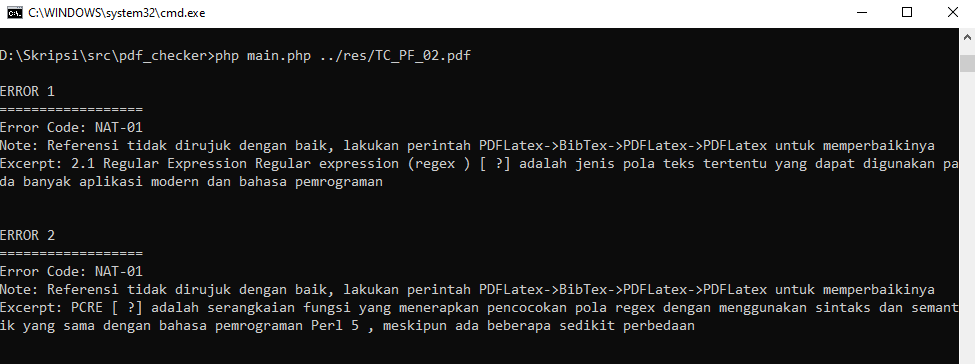
\includegraphics[scale=0.63]{uji_nat01.png}
	\caption{Laporan kesalahan fitur NAT-01}	
	\label{fig:ujinat01} 
\end{figure}

Laporan yang ditunjukan pada gambar \ref{fig:ujinat01} sudah sesuai dengan yang diharapkan.

\subsection{Menguji fitur VAN-03}
Hasil yang diharapkan dari pengujian fitur ini adalah perangkat lunak dapat menemukan kata ganti orang pada kalimat. Laporan kesalahan yang ditemukan pada \textit{test case} ''TC\_PF\_02.pdf'' dapat dilihat pada gambar \ref{fig:ujivan03}.

\begin{figure}[H]
	\centering	
	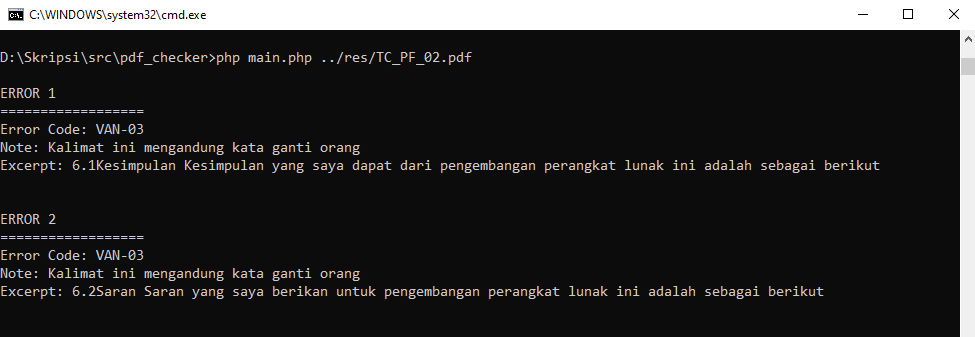
\includegraphics[scale=0.63]{uji_van03.png}
	\caption{Laporan kesalahan fitur VAN-03}	
	\label{fig:ujivan03} 
\end{figure}

Laporan yang ditunjukan pada gambar \ref{fig:ujivan03} sudah sesuai dengan yang diharapkan.

\section{Pengujian Eksperimental}
Pada pengujian eksperimental, perangkat lunak akan diuji dengan 5 buah \textit{test case} dokumen skripsi yang diambil dari \textit{Github} skripsi Informatika.